\documentclass{article}
\usepackage[T1]{fontenc}
\usepackage{iclr2027_conference,times}
\usepackage{amsmath,amssymb,amsthm,booktabs,graphicx,tabularx,xcolor,hyperref,etoolbox}
\hypersetup{colorlinks=true,linkcolor=blue!45!black,citecolor=blue!45!black,urlcolor=blue!45!black}
\newcommand{\E}{\mathbb{E}}
\newcommand{\Prob}{\mathbb{P}}
\newcommand{\pending}{\textit{Not run}}
\newcommand{\R}{\mathbb{R}}
\makeatletter
\patchcmd{\@maketitle}{Under review as a conference paper at ICLR 2027}{Working draft -- 5 September 2026 -- not submitted}{}{\errmessage{Draft header patch failed}}
\patchcmd{\@maketitle}{Anonymous authors}{Anonymous research draft}{}{\errmessage{Draft author patch failed}}
\patchcmd{\@maketitle}{Paper under double-blind review}{Empirical completion pending}{}{\errmessage{Draft status patch failed}}
\makeatother
\title{When Immediate Agreement Cannot Identify\ Persistent Preference}
\author{Anonymous authors}
\begin{document}
\maketitle

\begin{abstract}
Learning from a user's next message requires specifying what that message
measures. Immediate agreement may reflect a transient change in expression or
a persistent change in preference. We give an exact finite-state construction
in which these mechanisms induce the same historical observations, including
observed baseline states, but rank population actions differently under a
declared post-action matching objective. For a new user whose baseline state is
unavailable, the two-world expected-risk minimax regret is $2/15$. The result
does not apply unchanged when the deployment user's baseline state is observed,
and post-action matching is not itself a welfare criterion. Known, informative
delayed measurements identify the finite transition law under explicit
measurement assumptions. Existing constructed simulations show both benefits
and limitations of standard residual correction: a simpler anchor estimator can
outperform its propensity-weighted version in policy regret. We specify a
gated neural comparison with direct predictive and semantic controls. An initial
interface fails; one task-instruction repair qualifies, but training fails the
acquisition gate and the sparse methods remain unrun. A secondary public-data
audit yields an attrition-bound interval spanning both directions of change in
later reported attitudes. \textbf{This draft establishes neither neural method
superiority nor real assistant-induced preference change and is not currently
qualified for submission.}
\end{abstract}

\section{Introduction}
The next user message provides inexpensive supervision for an assistant, but
it is also a response to the assistant's own action. Hindsight self-distillation
conditions a teacher on that subsequent message and trains a student that did
not observe it \citep{sdpo}. Such training can be useful without making any
causal claim. A stronger claim---that the update improves a persistent user
preference---requires a connection between the observed utterance and a
specified persistent target. That connection cannot be inferred merely because
the user agrees with the preceding response.

Consider a recommendation followed by assent. The user may temporarily echo
the recommendation while retaining an earlier preference, or the recommendation
may change a preference that remains after the immediate conversational context
is removed. If both mechanisms generate the same observable logs, collecting
more of those logs cannot distinguish them. This ambiguity concerns the
measurement of latent state, in addition to familiar uncertainty about the
function used to predict an observed label. A delayed probe helps only when
its interpretation is justified independently: delay alone does not make a
report neutral, stable, or nonreactive.

This problem sits close to several established lines of work. SLIFT decomposes
feedback for selective learning \citep{slift}; PUMA models action-conditioned
user dynamics and inferred state \citep{puma}. Work on privileged likelihood
already separates loss or gradient fidelity from utility
\citep{privilegedlikelihood}. Human preference elicitation can change reported
preferences under a fixed underlying reward \citep{influencing}, and influenceable
reward functions raise competing normative objectives \citep{carroll2024}.
Our remaining question is specifically whether independent persistence
measurements resolve a consequential ambiguity for interaction learning. A
generic causal-personalization framing or a renamed residual estimator would
not establish a new contribution.

The present draft separates three objects. First, an exact witness establishes
observational nonidentification under a restricted decision setting. Second,
constructed finite-state simulations evaluate ordinary difference estimation;
they do not measure how frequently the ambiguity occurs among people. Third,
a prospective neural screen asks whether correction improves prediction of
stipulated delayed labels beyond simple learners receiving the same labels.
That predictive experiment is not an empirical test of the theorem's
action-induced state objective. Its completion and an externally defensible
measurement study remain necessary for the intended paper.

\section{Observed feedback and declared targets}
Let $Z_0$ be a baseline persistent state, $A$ an assistant action, $Z_1(A)$ the
persistent state after that action, and $S_1$ a transient expressed stance.
The observed next message $O$ is emitted from the latent state. In the exact
witness, the emission is the same in both mechanisms and simply reports $S_1$.
Historical data contain $(Z_0,A,O)$; thus the witness does not rely on hiding
the historical baseline state. The logging action has positive probability
under each baseline state.

We distinguish the value of an action that changes the target state,
\begin{equation}
 V_m(a)=\Prob_m\{a=Z_1(a)\}, \qquad m\in\{E,T\},
 \label{eq:causal-value}
\end{equation}
from the value of a predictive distribution for a fixed delayed label $B$,
\begin{equation}
 U(\pi)=\E[\pi(B\mid X)]. \label{eq:prediction-value}
\end{equation}
In Equation~\ref{eq:causal-value}, the evaluated action can change the state
that supplies its own reward. In Equation~\ref{eq:prediction-value}, the
evaluation label is fixed when the prediction is scored. Optimizing either
quantity is not automatically equivalent to protecting autonomy, consent,
pre-treatment preferences, or long-term welfare. Those require separately
defended objectives.

In the neural screen, $B$ is a constructed delayed-expression label on a held-out
task from an observed user cohort. The prediction is the full-vocabulary
probability of the native token for the correct option; other vocabulary tokens
receive zero credit. If $M(X)$ is the total probability of the four answer
tokens and $q(B\mid X)$ their normalized conditional probability, then
$\pi(B\mid X)=M(X)q(B\mid X)$. Consequently, both full-vocabulary NLL and
correct-token probability can improve solely by placing more mass on the answer
format. We report and gate conditional semantic correctness separately.

\section{A restricted identification witness}
Set $\Prob(Z_0=1)=3/5$ and log actions independently with probability $1/2$.
When an action conflicts with $Z_0$, let the user copy action zero with
probability one and action one with probability zero. In mechanism $E$, copying
changes expression only; in mechanism $T$, it changes persistent state as well.
The resulting immediate observation is $O=0$ when $A=0$ and $O=Z_0$ when $A=1$
in both mechanisms. Thus their complete historical laws are identical.

The action values under Equation~\ref{eq:causal-value} are
\begin{center}
\begin{tabular}{lcc}
\toprule
Mechanism & $V(0)$ & $V(1)$ \\
\midrule
Expression only $E$ & $2/5$ & $3/5$ \\
Persistent transition $T$ & $1$ & $3/5$ \\
\bottomrule
\end{tabular}
\end{center}
For a new anonymous user whose $Z_0$ is unavailable to the policy, let $q$ be
the learner's overall probability of action one, integrating over historical
data and any randomization. Identical historical laws imply the same $q$ in
both worlds. The expected regrets are $(1-q)/5$ and $2q/5$, so their maximum is
minimized at $q=1/3$, with regret $2/15$. This statement covers data-dependent
deterministic rules as well as randomized rules. A bound of $.2$ for every
deterministic learner would be false because the random historical sample
itself supplies randomization; Appendix~\ref{app:theory} gives a counterexample.

The deployment restriction matters. If the current user's $Z_0$ is observed,
the personalized rule $A=Z_0$ achieves value one in both witness worlds. The
historical mechanisms remain nonidentified, but this particular decision
problem no longer incurs regret. The construction therefore establishes neither
a universal personalization lower bound nor inevitable harm from adaptation.

A stipulated neutral probe maps $(Z_1,S_1)$ to $(Z_1,Z_1)$ without changing
$Z_1$. Adding its observation gives total variation distance $3/10$ between
the witness laws. More generally, with a known state-emission matrix $M$ of
full row rank, conditional probe distributions satisfy $Q_a=T_aM$ and identify
$T_a=Q_aM^\dagger$. This is standard linear identification, not a new general
matrix theorem. Unknown emission, missing action support, ill conditioning,
state-label ambiguity or probe-induced transitions change the conclusion.
Complete assumptions and proofs are in Appendix~\ref{app:theory}.

\section{Standard residual correction and fair information}
For a fixed model parameter $\theta$, let $g_i^{I}(\theta)$ be a proxy loss
gradient based on immediate feedback and $g_i^{D}(\theta)$ the corresponding
gradient under a valid delayed label. With $N$ immediate examples and a uniform
sample of $n$ paired delayed anchors, ordinary difference estimation uses
\begin{equation}
 \widehat g(\theta)=\frac1N\sum_{i=1}^{N}g_i^I(\theta)
 +\frac1n\sum_{i\in\mathcal A}\{g_i^D(\theta)-g_i^I(\theta)\}.
 \label{eq:difference}
\end{equation}
For fixed $\theta$ and the stated sampling design, the correction targets the
full delayed-gradient mean. Nonuniform selection requires the appropriate
known inclusion probabilities and support. This estimator belongs to classical
difference estimation and prediction-powered inference \citep{ppi}; the
arithmetic is not the proposed novelty.

The fixed-parameter identity does not establish a neural training guarantee.
Our SDPO-style teacher depends on the current adapter, is detached within an
update, and changes between updates. Reusing a fixed anchor set while adapting
parameters does not preserve an unconditional fixed-parameter unbiasedness
claim along the entire trajectory. Clipping a correction, clipping gradients,
finite optimization and selecting an action from an estimated value further
separate estimation bias from decision regret. Even an unbiased value estimate
need not induce a better decision than a biased estimate with favorable ranking.

Every sparse comparator must receive the same available immediate logs,
delayed labels and metadata. A full-delayed oracle is an extra-information
acquisition control, not an equal-budget baseline. Equal optimizer updates also
do not imply equal computation: the residual arm needs additional teacher and
student forwards. We report label access and computation separately and require
matched-compute comparisons before claiming method superiority.

\section{Existing constructed evidence}
\label{sec:finite}
The retained finite-state studies are developmental experiments on designed
cells. We recomputed their displayed aggregates directly from saved cell rows
and retained every relevant comparator. The first study uses 150 qualifying
design cells at each anchor budget, with 2,000 coupled synthetic draws per cell.
At 16 anchors per action, mean expression regret is $.08628067$ for immediate
feedback, $.01377017$ for ordinary anchors and $.00934317$ for clipped
augmentation. At 64 anchors the latter two values are $.00431483$ and
$.00268983$. These improvements are properties of this constructed screen, not
neural or human effect estimates.

\begin{figure}[t]
\centering
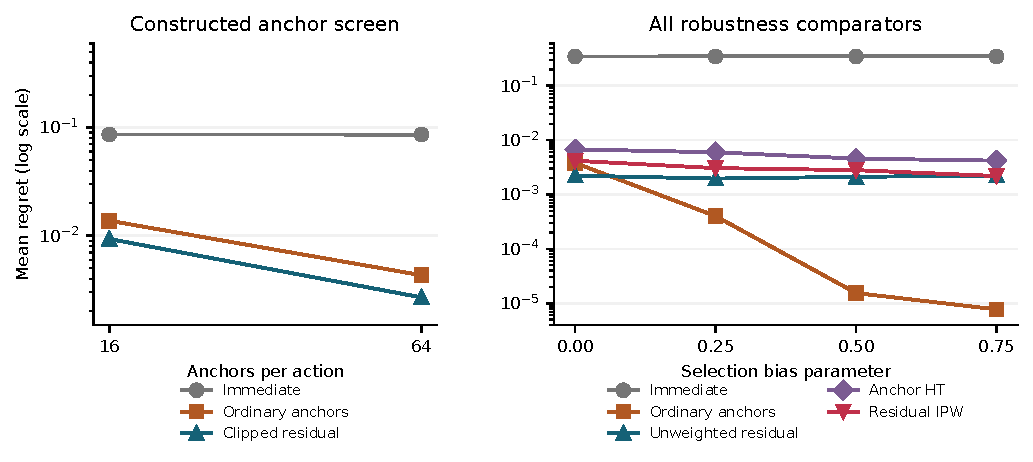
\includegraphics[width=\linewidth]{generated/finite_evidence.pdf}
\caption{Existing constructed simulations, recomputed from saved design-cell
rows. Left: 150 qualifying cells per budget. Right: all five comparators in
13 clean ranking-reversal cells per selection level. The logarithmic regret
axis preserves the raw comparator. Cells and coupled draws are not independent
human samples. Ordinary anchors can beat augmented IPW; unweighted augmentation
is best at random selection in this grid.}
\label{fig:finite}
\end{figure}

The robustness screen is more cautionary. Its clean ranking-reversal subset
contains 13 designed configurations per selection level. At random selection,
ordinary anchors have regret $.00380385$, better than augmented IPW at
$.00417692$, while unweighted augmentation is better than both at $.00222308$.
At the strongest included selection bias, ordinary anchors attain
$.00000769$ versus $.00218077$ for augmented IPW. The original bias-correction
checks still pass. The conclusion is that bias control and policy superiority
are distinct, and that omitting a simple comparator changes the interpretation.
Figure~\ref{fig:finite} shows all comparators rather than only the favorable pair.

A separate finite longitudinal calculation also rejects an automatic-harm
interpretation: symmetric adaptation need not increase mean baseline drift.
These retained results motivate sharper measurement and decision questions;
they do not jointly establish a successful learning method. Original protocols,
raw rows, replay receipts and corrected claim classifications remain preserved.

\section{Gated neural screen}
\label{sec:neural}
\paragraph{Status and population.}
The reduced screen stopped at acquisition. The task uses 630 learning
bases derived from PAHF and 96 development bases, with four option rotations
per base. The learning cohort has 20 source-user display-name groups; all 19
development groups occur in learning. The prepared data do not provide a
separate unique person identifier. We therefore target held-out tasks within this cohort, not
unseen-user generalization. The 256 reserved confirmation bases remain unopened
and are not consumed by preparation or development verification. The stipulated
old/new labels and transition narratives are constructed; they do not measure
assistant-caused human persistence.

\paragraph{Arms and budgets.}
Pool the existing four disjoint 16-base panels into one 64-base delayed-label
budget shared by all sparse learners. Each arm is one Qwen3.5-9B model with
the same immutable base revision, identical initial rank-eight adapter and a
fresh AdamW optimizer. Use 35 fixed updates at learning rate $10^{-4}$, no
weight decay, and the fixed final checkpoint. The population schedule visits
each learning base once, 18 rows per update. The anchor schedule presents two
bases in all four rotations per update: all 64 bases in the first 32 updates,
then six hash-selected revisits, totaling 280 anchor-row presentations.

\begin{table}[t]
\centering\small
\begin{tabularx}{\linewidth}{lXcc}
\toprule
Arm & Signal & Delayed bases & DEV result \\
\midrule
Raw & Immediate SDPO-style loss & 0 & Invalid \\
Full oracle & Delayed SDPO-style loss & 630 & Invalid \\
Anchor SFT & Pooled native-label NLL & 64 & \pending \\
Anchor SDPO & Pooled delayed teacher & 64 & \pending \\
Residual & Immediate plus paired correction & 64 & \pending \\
Mixture & $0.5$ immediate $+0.5$ anchor SDPO & 64 & \pending \\
\bottomrule
\end{tabularx}
\caption{Stagewise development screen. Raw and oracle ran but failed acquisition;
all four sparse arms remain unrun. Sparse arms would receive the same 630
immediate logs and 64 delayed bases. No method-superiority comparison is earned.}
\label{tab:neural}
\end{table}

The teacher loss is first-answer-token full-vocabulary
$\mathrm{KL}(p_\theta\Vert\operatorname{stopgrad}p_\theta^{\rm hindsight})$.
This is an SDPO-style adaptation, not a reproduction of the released
multi-token algorithm. Full-sequence SDPO and SLIFT given the same delayed
information belong to the conditional follow-up, not to an unearned baseline
claim in Table~\ref{tab:neural}.

\paragraph{Qualification and outcomes.}
The exact downstream serialization first undergoes a learning-only
16-base, four-rotation, two-context interface check. Every context/label cell
must have at least 14 of 16 correct conditional choices, mean target probability
at least $.70$ and mean answer mass at least $.10$. The raw and full-oracle arms
then run before any sparse arm. The oracle must improve old-target NLL by at
least $.10$ over both no-update and raw; raw must improve new-target NLL by at
least $.10$ over no-update. Every corresponding full-vocabulary and conditional
semantic probability change must be positive. Failure is an invalid acquisition
assay, not a causal negative.

If acquisition qualifies, the residual must improve old-target NLL by at least
$.03$, full-vocabulary correct-choice probability by $.02$, and conditional
semantic correctness by $.01$ against each of raw, anchor SFT, anchor SDPO and
the mixture. Probability gains must remain nonnegative in every rotation
stratum and leave-one-source-user-out aggregate. It must also beat each
prespecified cheap readout by more than $.005$ on both probability metrics.
Otherwise there is no basis to advance a neural-superiority claim. These are
practical development routing thresholds; they are not statistical equivalence
tests or validated neural power guarantees. A model-free stress audit invokes
the complete rule in 1,200 artificial studies with task and source-user
dependence. With no systematic residual advantage, 19 of 200 high-user-noise
studies pass, versus zero of 200 low-user-noise studies. These illustrative
routing frequencies are not calibrated false-positive rates for the neural
experiment. They reinforce the need for independent replication and a separately
specified confirmatory analysis.

\paragraph{Observed acquisition failure.}
The initial interface passes all eight cell-level accuracy/mass checks but
fails paired option-order stability (maximum target-probability range $.66690$).
It stops before training. One prospectively recorded repair adds the same
hypothetical preference-identification instruction to every neural prompt,
clarifying that listed product alternatives are stipulated rather than assessed
for technical feasibility. All 128 learning-only qualification choices then
match their targets. Labels, cases, budgets and numerical gates remain fixed.

After 35 updates per acquisition arm, oracle old-target NLL is $8.79766$ worse
than no-update, despite a $.02463$ correct-token probability gain. Raw new-target
NLL is $5.90668$ worse, despite a $.32009$ probability gain. The oracle's paired
probability range approaches one; the no-update DEV distribution also fails
its range guards. The run stops at 70 updates in 149.46 seconds on one GH200.
This is an invalid acquisition assay, not a negative result for residual
correction. It illustrates why one favorable endpoint cannot certify acquisition.

A post hoc diagnostic replays one outcome-blind selected 16-row batch per saved
checkpoint and reproduces all full logits exactly. On the original 128
learning qualification prompts, the final oracle teacher answers A throughout
and scores 32/128, versus the initial teacher's 128/128. Thus the saved adapter
has lost the initially demonstrated conditional capability. This diagnoses the
particular first-token training recipe; it neither isolates every cause nor
establishes a general failure of the released multi-token SDPO method.

\paragraph{Dependence, verification and stopping.}
Average rotations within base; retain source-user dependence in sensitivity
analysis. Check the exact expected IDs and semantic option mapping, rather
than accepting any complete-looking table. Paired per-base option-order ranges
and disagreement are required because global means can cancel opposing order
effects. The no-update comparator retains the mass and probability-range
requirements but is exempt from an argmax-disagreement gate: a uniform
stochastic distribution is a valid baseline despite arbitrary discrete ties.
Its disagreement is still reported. Record effective configurations, source and environment hashes,
resolved model/tokenizer and weight receipts, initialization and optimizer
states, raw logits, tokens and elapsed work. The original v2 verifier had a
wrong runner reference; a separate replay inspector binds the actual frozen
runner. It also found that floating-point profile-score ties depended on Python
hash iteration order. Exact rational arithmetic repairs the prospective control,
but the original controls are not retroactively certified. The amended receipt
explicitly distinguishes verified neural-acquisition evidence from an uncertified
full comparison. None of these repairs changes the failed acquisition decision.

A qualified negative parks this estimator at this budget. Interface failure
permits at most one isolated prospective repair. A pass permits independent
seeds, matched-compute controls and a second family, followed by fair published
baselines and one separately frozen confirmation. An identity in which delayed
and immediate text coincide is checked on CPU; a redundant 35-update training
arm is not counted as a transition experiment. No stage automatically turns
development success into a submission decision.

\section{External measurement and remaining evidence}
\label{sec:measurement}
A delayed response is an informative instrument only under an argued
measurement model. A credible external study needs randomized exposure,
comparable immediate and delayed measurements of the same declared construct,
a neutral comparison, repeated-measure stability or reactivity controls, and
prespecified delay and attrition handling. A new elicitation context may reveal
a different construct or cause a new transition. Repeated interaction can
confound retention of an earlier change with continued treatment.

Public data offer a narrower operational route. We inspected the public
release for \citet{costello2026canvassing}, which randomizes a conversation
about immigration versus smartphones. Its current processed cohort contains
1,108 records; an older public follow-up export uniquely matches 750 of them,
with 383 control and 367 treatment respondents. All eleven immediate and
follow-up item definitions match after whitespace normalization. The recorded
elapsed time from initial-study end to follow-up start is approximately
40--49 days (median 45.54), whereas the source manuscript states a 35-day mean.
This unresolved metadata discrepancy must remain visible in a reconstruction.
These are availability and linkage checks, not estimated response effects.

Such data can support a separately specified secondary analysis of later
\emph{reported attitudes}. They do not supply latent preference ground truth,
randomized measurement-reactivity controls, or an empirical bridge to the
action-induced target in Equation~\ref{eq:causal-value}. Roughly one third of
the processed cohort lacks follow-up, and postassignment exclusions prevent an
automatic intention-to-treat interpretation. A prospective analysis therefore
needs an explicit population, item-scoring rule and bounded-outcome attrition
sensitivity. The previously considered conspiracy-belief source
\citep{costello2024durably} has a 2026 editorial expression of concern concerning
its data pipeline \citep{thorp2026concern}; we do not treat its original public
release as a clean replication route.

We subsequently froze and executed a secondary numeric audit. Within the fixed
1,108-person processed cohort, the primary estimand is the change in recorded
treatment-minus-control prejudice-score contrast from immediate measurement to
the observed recontact round. Each of six items lies in $[0,100]$; allowing
every missing item its full range yields the sharp finite-cohort interval
$[-29.5053,36.3433]$. The policy-support analogue is $[-37.8035,28.5397]$.
These are identification intervals under range restrictions, not confidence
intervals or causal effects. They leave the direction unresolved and do not
establish absence of persistence. The 723 joint-complete prejudice respondents
give a descriptive contrast change of $+1.0377$; this selected subset cannot
replace the cohort bounds. All 49 prespecified missing-item departure settings
per scale and baseline completeness summaries are retained. No prediction,
demographic subgroup or persuasion-targeting analysis was performed.

The intended contribution remains conditional on a consequential learning
result and an honest external estimand. The strongest unresolved objection is
that the construction supplies better labels by assumption and applies a known
estimator. Passing a proxy-gradient gate, adding labels unavailable to baselines,
or selecting a favorable parser does not resolve that objection.

\section{Discussion and limitations}
The exact construction separates two latent mechanisms with identical immediate
observations. Its value is the explicit measurement and deployment assumptions,
not a claim that all personalization is nonidentifiable. The matrix recovery
argument and residual estimator are standard, and the finite-state evidence
already shows a simpler estimator can be better for decisions. No claim of
new general causal identification or general policy superiority follows.

The proposed neural screen measures fixed-label prediction on an observed
cohort. It cannot validate Equation~\ref{eq:causal-value}, identify human
persistence, or demonstrate welfare improvement. Its full decision rule has
undergone model-free stress checks and still needs empirical replication;
constructed Gaussian power for one marginal endpoint cannot qualify the whole
study. The same development data must not be used to repeatedly repair a
scientific failure until it passes. Submission is contingent on completing
the missing evidence, not on the existence of this draft.

\section*{Reproducibility statement}
The exact proofs are in the appendix. Displayed finite-state aggregates and
Figure~\ref{fig:finite} are generated from preserved cell rows with input hashes.
The corrected audit distinguishes formal claims, developmental simulations,
invalid assays, qualified negatives and unrun stages. A prospective protocol
and source freeze govern the reduced screen; immutable evidence and a separate
offline verifier are required for any eventual result. No anonymous artifact
URL is claimed before a concrete release exists.

\section*{Ethics statement}
Matching a post-action preference is not assumed to be welfare or consent.
Preference measurement can itself influence users. No new human study has been
conducted for this draft; any collection requires an appropriate consent,
review, privacy and follow-up plan before recruitment.

\section*{AI use statement}
AI systems assisted with hypothesis development, theoretical formulations and
proof checking, literature search, experimental design, code and test generation,
synthetic-data analysis, scientific interpretation and manuscript drafting.
This assistance includes substantive research contributions, not only language
editing. The human authors must verify all claims, sources and artifacts before
submission and remain responsible for them.

\bibliography{theory_sources}
\bibliographystyle{iclr2027_conference}
\clearpage
\appendix
% Input after \appendix. Requires amsmath, amssymb, and natbib.
% Bibliography entries are in paper/theory_sources.bib.
\section{Identification, restricted decision risk, and measurement assumptions}
\label{app:theory}

This appendix gives an exact counterexample and the assumptions under which
additional measurements resolve it. The example is a construction, not an
estimated model of human preferences. Its decision objective is one explicit
choice among objectives for influenceable preferences
\citep{carroll2024}. Neither the counterexample nor the sampling
identity below establishes a new general estimation method, human prevalence,
or a neural learning result.

\subsection{Two mechanisms with a common observation law}
\label{app:theory:witness}

Let a user's initial binary state be $Z_0\sim\operatorname{Bernoulli}(p)$.
A logging policy draws $A\in\{0,1\}$ with
$\Pr(A=1\mid Z_0=z)=e_z$. The post-action state is
$(P_1,S_1)$, where $P_1$ is the persistent component and $S_1$ is an expressed
stance. The initial state is $(Z_0,Z_0)$, and the common, action-independent
observation function is $O=S_1$. Fix copying probabilities $c_0,c_1\in[0,1]$.
If $A=Z_0$, both mechanisms leave the state unchanged. If $A\ne Z_0$,
the expression mechanism $E$ and the transition mechanism $T$ use
\begin{align}
 E:\quad (P_1,S_1)&=
 \begin{cases}(Z_0,A),&\text{with probability }c_A,\\
 (Z_0,Z_0),&\text{with probability }1-c_A;\end{cases}\\
 T:\quad (P_1,S_1)&=
 \begin{cases}(A,A),&\text{with probability }c_A,\\
 (Z_0,Z_0),&\text{with probability }1-c_A.\end{cases}
\end{align}
The labels ``persistent'' and ``expression'' are part of the construction.
They do not turn a recorded utterance into an independently measured state.

\paragraph{Proposition 1 (immediate observational equivalence).}
For any $p,e_0,e_1,c_0,c_1$, the joint law of $(Z_0,A,O)$ is identical under
$E$ and $T$. This remains true even if the historical log records $Z_0$ without
error and the action has randomized overlap.

\paragraph{Proof.}
When $a=z$, $\Pr(O=z\mid Z_0=z,A=a)=1$ in both mechanisms. When $a\ne z$,
both give $\Pr(O=a\mid Z_0=z,A=a)=c_a$ and
$\Pr(O=z\mid Z_0=z,A=a)=1-c_a$. Multiplying by the same initial-state and
logging probabilities proves equality of every joint atom. Hence the total
variation distance is zero. Any independent sample of historical logs, and
any statistic or randomized post-processing of that sample, has the same
law in the two worlds. This is equality by construction, not a test passed
by human data.\hfill$\square$

For a fresh user drawn independently from the same initial-state population,
define the value of an intervention that always chooses action $a$ by
\begin{equation}
 V_m(a)=\Pr_m\{a=P_1(a)\},\qquad m\in\{E,T\}.
 \label{eq:theory:persistent-value}
\end{equation}
The evaluated action itself may change the state against which it is scored.
This objective rewards post-action matching; it is not a definition of welfare
or a requirement to preserve the initial state. Direct evaluation gives
\begin{align}
 (V_E(0),V_E(1))&=(1-p,p),\\
 (V_T(0),V_T(1))&=(1-p+pc_0,\ p+(1-p)c_1).
\end{align}
For the exact witness $p=3/5$, $c_0=1$, $c_1=0$, these values are
\begin{equation}
 (V_E(0),V_E(1))=(2/5,3/5),\qquad
 (V_T(0),V_T(1))=(1,3/5).
 \label{eq:theory:witness-values}
\end{equation}
Thus action $1$ is uniquely optimal among constant actions in $E$, while
action $0$ is uniquely optimal in $T$. With $e_0=e_1=1/2$, the nonzero
immediate-log atoms $(z,a,o)$ have masses
\begin{equation}
 (0,0,0):1/5,\quad (0,1,0):1/5,\quad
 (1,0,0):3/10,\quad (1,1,1):3/10.
\end{equation}
The same equivalence also holds for the separately archived logging design
$(e_0,e_1)=(7/20,7/10)$; the logging designs must not be interchanged when
reporting a delayed-log total variation distance.

\subsection{The corrected expected-risk minimax statement}
\label{app:theory:minimax}

A learner receives $n$ independent historical immediate logs $D_n$ and may
use independent randomization $U$. It outputs one action $\delta(D_n,U)$ for
a fresh anonymous user. The fresh user's $Z_0$ is unavailable at deployment
and independent of $D_n,U$. The comparison class contains the two constant
actions. Define expected regret, averaging over training data and learner
randomization, by
\begin{equation}
 R_m(\delta)=\max_{a\in\{0,1\}}V_m(a)
             -\mathbb E_m[V_m(\delta(D_n,U))].
\end{equation}
This restriction is essential: it is not a lower bound for all personalized
policies with access to the current user's state.

\paragraph{Proposition 2 (two-point minimax risk).}
For the witness in Eq.~\eqref{eq:theory:witness-values}, for every $n\geq0$,
\begin{equation}
 \inf_\delta\max\{R_E(\delta),R_T(\delta)\}=\frac{2}{15},
 \label{eq:theory:minimax}
\end{equation}
where the infimum allows randomized learners. It is attained by ignoring
the data and choosing action $1$ with probability $1/3$.

\paragraph{Proof.}
By Proposition 1, $q=\Pr_m\{\delta(D_n,U)=1\}$ is the same under both
mechanisms. Equation~\eqref{eq:theory:witness-values} therefore gives
\begin{equation}
 R_E(\delta)=\frac15(1-q),\qquad
 R_T(\delta)=\frac25q.
\end{equation}
If $q\leq1/3$, the first expression is at least $2/15$; if $q\geq1/3$,
the second is at least $2/15$. At $q=1/3$ they are equal. The data-independent
randomized rule attains this probability for every sample size.\hfill$\square$

\paragraph{Correction: deterministic data dependence is not a fixed action.}
The minimum worst-case regret over the two \emph{fixed} deterministic actions
is $1/5$. The stronger assertion that every deterministic learning algorithm
has expected worst-case regret at least $1/5$ is false. For $n\geq1$, consider
the deterministic rule
\begin{equation}
 \delta(D_n)=\mathbf 1\{Z_{0,1}=0\},
\end{equation}
where $Z_{0,1}$ is the first historical user's initial state. In either world,
$q=2/5$. Its two expected regrets are $3/25$ and $4/25$, with maximum
$4/25<1/5$. The random historical sample supplies randomness even though the
algorithm has no random seed. Proposition 2 remains a lower bound for this
algorithm; no claim that the deterministic subclass attains $2/15$ at each
fixed finite $n$ is needed.

\paragraph{Observed-current-state escape.}
If the fresh user's $Z_0$ is observed before acting, the policy $A=Z_0$
causes no copying branch and has $A=P_1=Z_0$ with probability one under both
mechanisms. Its value is one and its regret against the optimal policy in
that enlarged class is zero. Historical mechanism nonidentification survives,
but the restricted anonymous-user decision lower bound no longer applies.
Likewise, the witness alone does not establish impossibility for an unknown
longitudinal system with other informative interventions or observations.

\subsection{What an additional measurement must identify}
\label{app:theory:measurement}

In the binary construction, define an ideal neutral probe by the state map
$(P_1,S_1)\mapsto(P_1,P_1)$ followed by the same emission function. Its
output is $B=P_1$. The only immediate-log atom whose delayed outcome differs
between the witness worlds is $(Z_0,A,O)=(1,0,0)$: it has $B=1$ in $E$ and
$B=0$ in $T$. Consequently, the total variation distance between the extended
laws of $(Z_0,A,O,B)$ is $3/10$ under balanced randomized logging, and
$(3/5)(1-7/10)=9/50$ under the archived state-dependent logging design.
The probe identifies these two stipulated worlds because its exclusion and
measurement properties were specified, not because time elapsed.

The following finite-state statement makes the measurement requirement
explicit. Let $Z_0$ and $P_1$ take values in $\{1,\ldots,r\}$ and let
$T_a(z,j)=\Pr(P_1=j\mid Z_0=z,\operatorname{do}(A=a))$. Assume that:
\begin{enumerate}
 \item the baseline states being conditioned on are observed without error,
 have positive probability, and the logged action is randomized conditional
 on these states with positive probability for each relevant action;
 \item the probe does not change $P_1$, which remains stable over the specified
 horizon; and its known measurement law is the row-stochastic matrix
 $M_{jb}=\Pr(B=b\mid P_1=j)$, with no remaining direct dependence on action,
 baseline, or transient expression conditional on $P_1$;
 \item the full-population conditional probe distributions are observed or
 recoverable under an explicitly justified sampling and response model.
\end{enumerate}
Randomizing invitations to a delayed survey does not by itself justify the
third condition when actual response depends on the unobserved outcome.

\paragraph{Proposition 3 (known-emission identification).}
Writing $Q_a(z,b)=\Pr(B=b\mid Z_0=z,A=a)$, these assumptions give
$Q_a=T_aM$. If $M$ has full row rank $r$, then
\begin{equation}
 T_a=Q_aM^+,\qquad
 \|\widehat T_a-T_a\|_F
 \leq\|\widehat Q_a-Q_a\|_F\,\|M^+\|_2,
 \quad \widehat T_a=\widehat Q_aM^+,
 \label{eq:theory:known-emission}
\end{equation}
where $M^+$ is its Moore--Penrose inverse. The error bound assumes $M$ is
known exactly; it does not account for estimating or misspecifying $M$.

\paragraph{Proof.}
Conditioning on $P_1$ gives $Q_a=T_aM$. Full row rank implies $MM^+=I_r$,
so right multiplication identifies $T_a$. Submultiplicativity of the
Frobenius and spectral norms proves the error bound.\hfill$\square$

Small singular values can make finite-sample inversion unstable. Full row
rank is a sufficient condition here, not a claim that every target functional
requires full transition identification. Conversely, for
\begin{equation}
 M=\begin{pmatrix}1&0\\0&1\\0&1\end{pmatrix},\qquad
 T^{(1)}=I_3,\qquad
 T^{(2)}=\begin{pmatrix}1&0&0\\0&0&1\\0&1&0\end{pmatrix},
\end{equation}
$T^{(1)}M=T^{(2)}M$ although $T^{(1)}\ne T^{(2)}$. Thus additional probe
samples alone do not fix a measurement channel that aliases these states.
An unknown emission matrix also leaves a factorization problem; this theorem
does not learn or validate it from arbitrary conversational logs.

\subsection{The standard residual estimator and its limits}
\label{app:theory:residual}

For one randomized action stratum, let the finite population of $N$ logged
units have immediate agreement scores $O_i\in[0,1]$ and delayed scores
$B_i\in[0,1]$. The target here is the finite-population mean
$\overline B_N=N^{-1}\sum_i B_i$. Let $S$ be a uniformly selected subset of
$k$ units, sampled without replacement, on which both scores are observed.
Then the difference estimator is
\begin{equation}
 \widehat\mu_{\rm diff}=\overline O_N+
 \frac1k\sum_{i\in S}(B_i-O_i).
 \label{eq:theory:difference}
\end{equation}
It is standard model-assisted estimation, closely related to the mean
estimator in prediction-powered inference
\citep{ppi,mozer2026difference}.

\paragraph{Proposition 4 (design expectation).}
Conditional on the complete finite population,
$\mathbb E_S[\widehat\mu_{\rm diff}]=\overline B_N$. More generally, if
$R_i$ indicates that unit $i$ is measured and its positive inclusion
probability $\pi_i=\Pr(R_i=1\mid\{O_j,B_j\}_{j=1}^N)$ is known, then
\begin{equation}
 \widehat\mu_{\rm HT-diff}=\frac1N\sum_{i=1}^N
 \left[O_i+\frac{R_i}{\pi_i}(B_i-O_i)\right]
 \label{eq:theory:ht-difference}
\end{equation}
has the same conditional expectation. Dependence among the $R_i$ does not
change this expectation identity, although it matters for variance.

\paragraph{Proof.}
In the first design, $\mathbb E[\mathbf1\{i\in S\}]=k/N$; linearity gives
$\mathbb E[k^{-1}\sum_{i\in S}(B_i-O_i)]
=N^{-1}\sum_i(B_i-O_i)$. In the second design,
$\mathbb E[R_i/\pi_i]=1$ for each unit. Adding $\overline O_N$ yields
$\overline B_N$ in each case.\hfill$\square$

For a superpopulation response model using observed covariates $W$, a
corresponding sufficient condition is
$\mathbb E[R\mid B,O,W]=\pi(W)>0$ with known $\pi(W)$. A randomized
invitation probability is not the full measurement-inclusion probability
if nonresponse is selective. Plug-in estimated weights, self-normalization,
outcome-dependent selection with unknown probabilities, and fitting a proxy
on the same sampled labels require their own analysis; Proposition 4 does
not supply a blanket finite-sample unbiasedness guarantee for them.

\paragraph{Clipping changes the expectation.}
The archived first finite-state implementation clips
$\widehat\mu_{\rm diff}$ to $[0,1]$. This can reduce squared error for a
target in $[0,1]$, but does not preserve unbiasedness. For the finite
population $N=2$, $k=1$, $(O_1,O_2)=(1,0)$ and $(B_1,B_2)=(0,0)$,
Eq.~\eqref{eq:theory:difference} equals $-1/2$ or $1/2$ with equal
probability. Its expectation is the true mean zero. After clipping, the
expectation is $1/4$. This counterexample concerns estimator expectation;
it does not invalidate a properly reported Monte Carlo regret comparison.

\paragraph{Unbiasedness does not imply a decision advantage.}
For independent identically distributed pairs with finite second moments,
the same $k$ uniformly selected labels from $N$ pairs, and coefficient one,
direct covariance expansion gives
\begin{equation}
 \operatorname{Var}(\widehat\mu_{\rm diff})
 =\frac{\operatorname{Var}(B)}{k}
 +\left(\frac1k-\frac1N\right)
 \left[\operatorname{Var}(O)-2\operatorname{Cov}(B,O)\right].
\end{equation}
Here $\operatorname{Var}(\overline O_N)=\operatorname{Var}(O)/N$,
$\operatorname{Var}(\overline{B-O}_S)=\operatorname{Var}(B-O)/k$, and
$\operatorname{Cov}(\overline O_N,\overline{B-O}_S)
=\operatorname{Cov}(O,B-O)/N$, which proves the formula. Thus the estimator
need not beat the ordinary mean of the same $k$ delayed labels. Smaller
estimation error also need not change which action is selected, and a biased
estimator can have smaller decision regret on a particular population.
All same-label anchor means and simple shrinkage/mixture baselines therefore
belong in a method comparison. In the constructed truthful-transition world
$B_i=O_i$ for every pair, so its correction is identically zero; observing
this equality in a replay is an algebra check, not an independent empirical
discovery about human behavior.

\subsection{The empirical target is a separate estimand}
\label{app:theory:bridge}

The constructed EndoPAHF assay assigns a historical interaction an immediate
label and a stipulated delayed label. It then scores a later model answer
against that fixed label. No state-transition kernel is applied to the
\emph{evaluated} later answer. Its expected correct-label score has the form
\begin{equation}
 U_B(\theta)=\mathbb E_{(X,B)\sim\mathcal D}
                   [\pi_\theta(B\mid X)],
 \label{eq:theory:predictive-target}
\end{equation}
with a fixed constructed distribution $\mathcal D$. If $\pi_\theta$ is a
full-vocabulary next-token distribution, all tokens other than the native
correct answer token receive reward zero; a constrained option-normalized
policy instead defines a different decision rule and must be labeled as such.
Neither version equals Eq.~\eqref{eq:theory:persistent-value} merely because
the label is called delayed. Established users appearing in both learning
and evaluation also do not become unseen users when the query prefix changes.

Replacing $(B_i,O_i)$ in the residual identity by fixed, differentiable
delayed and immediate losses can identify the corresponding sampled loss
or its gradient when the same sampling conditions hold and differentiation
commutes with expectation. It does not prove that this gradient improves
Eq.~\eqref{eq:theory:predictive-target}, let alone an action-dependent human
state objective. Feedback generated from the learner's own policy adds
distributional derivatives not supplied by a fixed-target identity.
The distinction between likelihood, held-out feedback gradients, and value
is already central to \citet{privilegedlikelihood}.

Finally, an immediate-versus-delayed human survey study can identify effects
on a specified measured response under randomization and justified attrition
assumptions. It cannot establish $B=P_1$, a known full-rank $M$, absence of
measurement reactivity, or a uniquely correct welfare objective simply by
having a follow-up date. Those are separate validation and normative tasks.

\section{Complete constructed comparison}
\begin{center}\small
\begin{tabular}{rrrrrr}
\toprule
Selection & Immediate & Anchors & Residual & Anchor HT & Residual IPW \\
\midrule
0.00 & 0.34567308 & 0.00380385 & 0.00222308 & 0.00676538 & 0.00417692 \\
0.25 & 0.34592308 & 0.00040000 & 0.00196154 & 0.00596923 & 0.00305385 \\
0.50 & 0.34596154 & 0.00001538 & 0.00211154 & 0.00456923 & 0.00280385 \\
0.75 & 0.34582692 & 0.00000769 & 0.00223846 & 0.00418846 & 0.00218077 \\
\bottomrule
\end{tabular}
\end{center}

The selected subsets match the original declared design predicates. Their
averages do not estimate population prevalence. Complete raw cells and
unselected diagnostics remain in their historical evidence roots.
\end{document}
